\chapter{Frame representations}\label{AppendixA}
\section{Constraints}\label{app:constraints}
\ex.\label{app:const:proper}\textit{proper-scale} $\und$ \textit{measure-of-change} $\rightarrow \bot$

\ex.\label{app:const:temp:amount}\textit{amount} $\und$ \textit{temperature} $\rightarrow \bot$

\ex.\label{app:const:card}\textit{event $\und$ cardinality $\rightarrow$ iteration}

\ex.\label{app:constr:duration}\textit{bounded-event} $\und$ \DURATION .$\top$ $\rightarrow$ (\MDIM .\textit{measure-of-change} $\und$ time) $\und$  \MDIM .\MIN = 0 $\und$ \MDIM .\MAX $\triangleq$ \DURATION .\VAL

\ex.\label{app:rule:minmaxevent}\a. \MIN .$\top$ $\und$ \INIT .$\top$ $\rightarrow$ \INIT .\POS $\triangleq$ \MIN
\b. \MAX .$\top$ $\und$ \FIN .$\top$ $\rightarrow$ \FIN .\POS $\triangleq$ \MAX

\section{Prefixes}\label{app:pref}

\begin{figure}[H]
\centering
\begin{forest}
[VP\textsuperscript{[E=\textbf{f}]}
  [Pref [za-]]
  [VP\textsuperscript{[E=\textbf{e}]}]
]
\end{forest}
\begin{tabular}[t]{ll}
\begin{tabular}[t]{l}
\avm{
\btag{f} [\type*{transition}
      \POST & [\type*{event}
         \MDIM & [\type*{proper-scale}
            \MIN & deg ] 
     ]
   ]
}
\end{tabular}
\begin{footnotesize}
\begin{tabular}[t]{l}
$\tuple{\btag{f}\BC\POST,\btag{e}}\D\type{esegm-of}$\\[1ex]
$\tuple{\btag{f}\BC\POST\C\MDIM,\btag{e}\BC\MDIM}\D\type{segm-of}$\\
\end{tabular}
\end{footnotesize}
\\\\
\begin{tabular}[t]{l}
\avm{
\btag{e} [\type*{event}
	 \VERBDIM & \1\\
     \MDIM & \1 [\type*{proper-scale}]
   ]
}
\hfill
\end{tabular}
\end{tabular}
\hfill
\caption{Representation of the contribution of the prefix \textit{za-}}
\label{app:za.frame.semantics}
\end{figure}

\begin{figure}[H]
\begin{minipage}{0.4\textwidth}
\avm{
\btag{e} [\type*{bounded-event}
	   \NOUNDIM & \3\\       
	   \VERBDIM & \3\\
       \MDIM & \3[\type*{scale}
			\MIN & \1 \\	  
			\THRESHOLD & \2
       ] \\
       \INIT & [\type*{stage}
     		\POS & \1]\\
      \FIN & [\type*{stage} 
  		 	\POS & \4 ]\\
   ]
}\\
\vspace{1cm}
\centering
\svar{2} $\leq$ \svar{4}
\end{minipage}
\hfill
\begin{minipage}{0.4\textwidth}
\begin{forest}
[VP\textsuperscript{E=\textbf{e}}
  [Pref [na-]]
  [VP\textsuperscript{[E=\textbf{e}]}]
]
\end{forest}
\end{minipage}
\caption{Representation of the contribution of the prefix \textit{na-}\label{app:na}}
\end{figure}

\begin{figure}[H]
% \begin{minipage}{0.4\textwidth}
\avm{
\btag{e} [\type*{bounded-event}
   	   \VERBDIM & \1\\
       \MDIM & \1 [\type*{scale}] \\
       \INIT & [\type*{stage}
     		\POS & \2]\\
       \FIN & [\type*{stage} 
  		 	\POS & \3 ]\\
   ]
}\hfill%
% \end{minipage}
% \begin{minipage}{0.55\textwidth}
\avm{
\btag{e}  [\type*{bounded-event}
   \NOUNDIM & \3\\
    \MDIM & \3 [
       \type*{closed-scale $\und$ proper-scale}
       \MIN & \1\\
       \MAX & \2]\\
    \INIT & [\type*{stage}
       \POS & \1 ]\\
     \FIN & [\type*{stage}
       \POS & \2 ]
  ]
}
% \end{minipage}
%% Add requirement that if m-dim = path, path-start = init
\caption{Frame representations of the prefix \textit{po-} (left) and of of the prefix \textit{pere-} for the closed scale case (right) \label{app:po:delim}}
\end{figure}

\begin{figure}[H]\small
\begin{minipage}{0.5\textwidth}
\avm{
\btag{e} [\type*{bounded-event}
  	\NOUNDIM & \4\\
    \MDIM & \4 [
       \type*{proper-scale $\und$}\type*{one-marked-point}
       \MARKED & \2 ]\\
    \INIT & [\type*{stage}
       \POS & \1 ]\\
     \FIN & [\type*{stage}
       \POS & \3 ]\\
  ]
}\\
\centering
\svar{1} $<$ \svar{2} $<$ \svar{3}
 \end{minipage}\hfill%
 \begin{minipage}{0.45\textwidth}
\avm{
\btag{f}  [\type*{bounded-event}
     \MDIM & \3 [\type*{property-scale} ]\\
     \NOUNDIM & \4\\
     \INIT &  \1\\
     \FIN &  \2 \\
     \MANN & \5\\
     \PREP & \btag{e} [\type*{event}
  	 	\THEME & \6\\
        \MDIM & \3\\
    	\NOUNDIM & \4\\
    	\INIT &  \1\\
     	\FIN &  \2 \\
     	\MANN & \5
     ]
  ]
 }
 \end{minipage}
\caption{Frame representation of the prefix \textit{pere-}: case of a one marked point scale on the left and case of a property scale on the right \label{app:pere:iter}}
\end{figure}

\begin{figure}[H]\small
\begin{minipage}{0.45\textwidth}
\avm{
\btag{f} [\type*{bounded-event}
   		\MANN & \4\\
   		\ACTOR & \5\\
  	 	\THEME & \9\\
        \MDIM & [ \type*{closed-scale}\type*{$\und$ property-scale}
			\MIN & \2\\
			\MAX & \1						
        ]\\
    	\INIT & [\type*{stage}
    		\POS &  \3]\\
     	\FIN &  [\type*{stage}
    		\POS &  \1]\\
     	\PARTOF & \btag{e}\\
       \NOUNDIM & [\7]\\
       \VERBDIM & [\8]
    ]
 }
 \end{minipage}\hfill%
 \begin{minipage}{0.45\textwidth}
\avm{
\btag{e} [\type*{bounded-event}
   		\MANN & \4\\
   		\ACTOR & \6\\
  	 	\THEME & \9\\
        \MDIM & [ \type*{closed-scale}\type*{$\und$ property-scale}
			\MAX & \1						
        ]\\
    	\INIT &  [\type*{stage}
    		\POS &  \2]\\
     	\FIN &  [\type*{stage}
    		\POS &  \1]\\
       \NOUNDIM & [\7]\\
       \VERBDIM & [\8]
    ]
 }\\
 \vspace{0.5em}
 \centering
$\tuple{\btag{f}\BC\MDIM,\btag{e}\BC\MDIM}\D\type{segm-of}$\\[1ex]
\end{minipage}
\caption{Frame representation of the prefix \textit{do-} \label{app:do}}
\end{figure}

\pagebreak

\section{Verbs}\label{app:verbs}
\begin{figure}[H]
% \begin{minipage}{0.32\textwidth}
\avm{
\btag{e} [\type*{transloc}
	   \MANN & [\type*{run}]\\
       \ACTOR & \1\\
	   \TRACE & \2
]
}\hfill%
% \end{minipage}
% \begin{minipage}{0.33\textwidth}
\avm{
\btag{e} [\type*{transloc}
	   \MANN & [\type*{fly}]\\
       \ACTOR & \1\\
	   \TRACE & [\type*{trace}]\\
	   \PATH & \2 [\type*{path}]\\
	   \VERBDIM & \2\\
	   \MDIM & \2
]
}\hfill%
% \end{minipage}
% \begin{minipage}{0.3\textwidth}
\avm{
\btag{e} [\type*{transloc}
	   \MANN & [\type*{run}]\\
       \ACTOR & \1\\
	   \TRACE & [\type*{trace}]\\
	   \PATH & \2 [\type*{path}]\\
	   \VERBDIM & \2\\
	   \MDIM & \2
]
}%
% \end{minipage}
\caption{Verbs \textit{begat'}$^{\INDET}$ `to run' (left), \textit{letat'}$^{\DET}$ `to fly' (center), and \textit{be\v{z}at'}$^{\DET}$ `to run' (right)}
\end{figure}

\begin{figure}[H]\small
% \begin{minipage}{0.48\textwidth}
\avm{
 \btag{e} [\type*{state}
  		\STATE & [\type*{be\_seen}]\\
  		\THEME & \1 [
  			\COLOR & [\type*{yellow}]\\
  		]\\
  		\VERBDIM & \btag{e}
  ]
}\hfill%
% \end{minipage}
% \begin{minipage}{0.47\textwidth}
\avm{
\btag{e} [\type*{change-of-state}
  \VERBDIM & \2 [\type*{property-scale}\type*{$\und$ yellow} 
  	\MIN & \3\\
  	\MAX & \4  
  ]\\
  \MDIM & \2\\
  \THEME & \1
]
}%
% \end{minipage}
\caption{Two interpretations of the verb \textit{\v{z}eltet'} `to be yellow and be seen/to become yellow' \label{app:zeltet}}
\end{figure}

\begin{figure}[H]\small
% \begin{minipage}{0.3\textwidth}
\avm{
\btag{e} [\type*{event $\und$iteration}
    \MANN & [\type*{burst}]\\
    \ACTOR & \1\\
    \THEME & \2\\
    \VERBDIM & \btag{e}
  ]
}\hfill%
% \end{minipage}
% \begin{minipage}{0.35\textwidth}
\avm{
\btag{e} [\type*{process}
	   \MANN & [\type*{cook}]\\
       \ACTOR & \2\\
	   \THEME & [\type*{food}
	   		\AMOUNT & \1 ]
]
}\hfill%
% \end{minipage}
% \begin{minipage}{0.3\textwidth}
\avm{
\btag{e} [\type*{process}
    \MANN & [\type*{live}]\\
    \ACTOR & \1\\
    \VERBDIM & \btag{e}\\
    \MDIM & \btag{e}
  ]
}%
% \end{minipage}
\caption{Verbs \textit{lopat'} `to burst' (left), \textit{varit'} `to cook' (center), and \textit{\v{z}it'} `to live' (right) \label{app:frame:lopat}}
\end{figure}

\begin{figure}[H]
% \begin{minipage}{0.48\textwidth}
\avm{
\btag{e} [\type*{change-of-state}
	   \MANN & [\type*{heat}]\\
       \ACTOR & \1\\
	   \THEME & \2\\
	   \VERBDIM & \3 [\type*{temperature}]\\
	   \MDIM & \3
]
}\hfill%
% \end{minipage}
% \begin{minipage}{0.47\textwidth}
\avm{
  \btag{e} [\type*{process $\und$ closed-scale}
    \MANN & [\type*{spend-time $\und$ winter}]\\
    \ACTOR & \1\\
    \VERBDIM & \btag{e}\\
    \MDIM & \btag{e}\\
    \MIN &  [\type*{winter-start}]\\
    \MAX &  [\type*{winter-end}]\\
  ]
}%
% \end{minipage}
\caption{Verbs \textit{gret'} `to heat' (left) and  \textit{zimovat'} `to spend winter time' (right) \label{app:live}}
\end{figure}


\section{Nouns}\label{app:nouns}
\begin{figure}[H]\small
% \begin{minipage}{0.6\textwidth}
\avm{
\btag{f} [\type*{soup}
	   \AMOUNT & [\type*{amount}
	   		\VAL & \1\\
	   		\MUNIT & ml ] \\
       \TEMP & [\type*{temperature}
	   		\VAL & \2\\
	   		\MUNIT & °C ] \\
       \KIND & [\type*{soup-kind}]\\
       \TASTE & [\type*{taste}]\\
       \AMOUNTDIM & [\type*{amount $\und$}\type*{measure-of-change}
       		\MIN & 0\\
       		\MAX & \1
       	]\\
       	\TEMPDIM & [\type*{temperature $\und$}\type*{proper-scale}
       		\MIN & \2\\ 
       		\MAX & 100
       	]
]
}\hfill%
% \end{minipage}
% \begin{minipage}{0.35\textwidth}
\avm{
\btag{g} [\type*{match}
	   \DURATION & \1\\
	   \GAME & [\type*{game}]\\
	   \PLAYERS & [\type*{entity}
	   		\CARD & \2
	   ] 
]
}%
% \end{minipage}
\caption{Nouns \textit{sup} `soup' (left) and \textit{partija} `match' (right)}
\end{figure}

\begin{figure}[H]
% \begin{minipage}{0.3\textwidth}
\avm{
\btag{f} [\type*{road}
	   \WIDTH & \1\\
	   \LOC & \2\\
	   \EDGE & \3
]
}\hfill%
% \end{minipage}
% \begin{minipage}{0.3\textwidth}
\avm{
\btag{f} [\type*{hurricane}
	   \TIME & \1\\
	   \LOC & \2\\
	   \NAME & \3
]
}\hfill%
% \end{minipage}
% \begin{minipage}{0.35\textwidth}
\avm{
\btag{f} [\type*{balloon}
	   \CARD & [\type*{cardinality}
       		\POS & \1
       	]\\
       \SIZE & \2\\
       \COLOR & \3
]
}%
% \end{minipage}
\caption{Nouns \textit{doroga} `road' (left), \textit{uragan} `hurricane' (center), and \textit{\v{s}ar} `balloon' (right) \label{app:road}}
\end{figure}

\section{Measure phrases}\label{app:measure}
\begin{figure}[H]
\begin{tabular}[t]{c}
\begin{forest}
[NumP\textsuperscript{[I=\textbf{f}]}
[Num] [N]
]
\end{forest}\\
\avm{
\btag{f} [\type*{length}
  		\VAL & 2\\
  		\MUNIT & hour  
  ]
}
\end{tabular}
\hfill
\begin{tabular}[t]{c}
% % 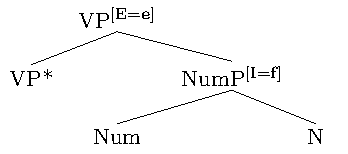
\includegraphics[scale=1]{VNumP.pdf}\\
\begin{forest}
[VP\textsuperscript{[E=\textbf{e}]}
  [VP*]
  [NumP\textsuperscript{[I=\textbf{f}]}
    [Num] [N]
  ]
]
\end{forest}\\
\avm{
\btag{e}[\type*{event}
  \DURATION & \btag{f}[\type*{length}
  		\VAL & 2\\
  		\MUNIT & hour  
  ]
]
}
\end{tabular}
\caption{Frame representation of the time adverbial \textit{2 \v{c}asa} `for 2 hours' before and after enriching its structure \label{app:2hours}}
\end{figure}

\section{Constructors}\label{app:constructors}

\begin{figure}[H]
\begin{minipage}{0.6\textwidth}
\avm{
\btag{e} [\type*{event}
	\THEME & \btag{f} [\type*{entity}
       	\TEMPDIM & \1
	]\\
	\NOUNDIM & \1
]
}
\end{minipage}
\begin{minipage}{0.35\textwidth}
\begin{tikzpicture}[baseline]
\node at (0,0) (VP) {VP\textsuperscript{[E=\textbf{e}]}};
\node (follows) [right = 1em of VP] {$\prec\prec$};
\node [right = 1em of follows] (NP) {NP\textsuperscript{[I=\textbf{f}]}};
\node [below=\baselineskip of NP] (N) {N};
\draw (NP) -- (N);
\end{tikzpicture}
\end{minipage}
\caption{Temperature dimension constructor\label{app:temp}}
\end{figure}

\begin{figure}[H]
\begin{minipage}{0.5\textwidth}
\avm{
\btag{e} [\type*{event}
	\THEME & \btag{f} [\type*{entity}
       \AMOUNTDIM & \1
	]\\
\NOUNDIM & \1
]
}
\end{minipage}
\begin{minipage}{0.4\textwidth}
% % 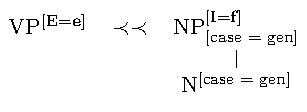
\includegraphics[scale=1]{NPgen.pdf}
\begin{tikzpicture}[baseline]
\node at (0,0) (VP) {VP\textsuperscript{[E=\textbf{e}]}};
\node (follows) [right = 1em of VP] {$\prec\prec$};
\node [right = 1em of follows] (NP) {NP$^{\text{[I=\textbf{f}]}}_{\text{[case = gen]}}$};
\node [below=\baselineskip of NP] (N) {N\textsuperscript{[case = gen]}};
\draw (NP) -- (N);
\end{tikzpicture}
\end{minipage}
\caption{Amount dimension constructor \label{app:amount}}
\end{figure}

\begin{figure}[H]
\small
% \begin{minipage}{0.575\textwidth}
\avm{
\btag{e} [\type*{event}
	\THEME & \btag{f} [\type*{entity}
       \CARD & [\type*{cardinality}
       		\POS & \1
       	]
	]\\
\MDIM & [\type*{cardinality}
			\MIN & 0\\
       		\MAX & \1
       	]
]
}
% \end{minipage}
\hfill%
\begin{minipage}[c]{0.4\textwidth}
% % 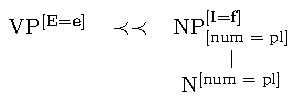
\includegraphics[scale=1]{NPpl.pdf}
\begin{tikzpicture}[baseline]
\node at (0,0) (VP) {VP\textsuperscript{[E=\textbf{e}]}};
\node (follows) [right = 1em of VP] {$\prec\prec$};
\node [right = 1em of follows] (NP) {NP$^{\text{[I=\textbf{f}]}}_{\text{[num = pl]}}$};
\node [below=\baselineskip of NP] (N) {N\textsuperscript{[num = pl]}};
\draw (NP) -- (N);
\end{tikzpicture}
\end{minipage}
\caption{Cardinality dimension constructor \label{app:cardinality}}
\end{figure}

\begin{figure}[H]
\begin{minipage}{0.4\textwidth}
\avm{
\btag{e} [ \type*{event}
	\PATH & \1 [ \type*{path}
		\MIN & \2\\
		\MAX & \3
	]
]
}\\
\centering
\svar{1} $\in$ \svar{5} $\und$ \svar{2} $\in$ \svar{4} $\und$
\svar{3} $\in$ \svar{4}
\end{minipage}\hfill%
% \begin{minipage}{0.2\textwidth}
\avm{
\btag{f} [\type*{landmark}
       	\EDGE & \4 \\
       	\LOC & \5 ]
}\hfill%
% \end{minipage}
% \begin{minipage}{0.35\textwidth}
\begin{tikzpicture}[baseline]
\node at (0,0) (VP) {VP\textsuperscript{[E=\textbf{e}]}};
\node (follows) [right = 1em of VP] {$\prec\prec$};
\node [right = 1em of follows] (NP) {NP\textsuperscript{[I=\textbf{f}]}};
\node [below=\baselineskip of NP] (N) {N};
\draw (NP) -- (N);
\end{tikzpicture}
% \end{minipage}
\caption{Path dimension constructor \label{app:path}}
\end{figure}

\begin{figure}[H]
\small
\begin{minipage}{0.42\textwidth}
\avm{
\btag{e} [\type*{event}
	\NOUNDIM & [ \type*{time $\und$}\type*{one-point-scale}
			\MARKED & \1
	 ]
]
}
\end{minipage}
\begin{minipage}{0.18\textwidth}
\avm{
\btag{f} [\type*{entity}
       	\TIME & \1]
}
\end{minipage}
\begin{minipage}{0.35\textwidth}
\begin{tikzpicture}[baseline]
\node at (0,0) (VP) {VP\textsuperscript{[E=\textbf{e}]}};
\node (follows) [right = 1em of VP] {$\prec\prec$};
\node [right = 1em of follows] (NP) {NP\textsuperscript{[I=\textbf{f}]}};
\node [below=\baselineskip of NP] (N) {N};
\draw (NP) -- (N);
\end{tikzpicture}
\end{minipage}
\caption{Time scale constructor: case of one marked point \label{app:time}}
\end{figure}

\begin{figure}[H]
% \begin{minipage}{0.7\textwidth}
\hfill\avm{
\btag{e}  [\type*{bounded-event}
     \MDIM & \3 [\type*{property-scale $\und$ closed-scale} 
		\MIN & \1\\
		\MAX & \2      
      ]\\
     \NOUNDIM & \3\\
     \INIT &  [\type*{stage}
     	\POS & \1]\\
     \FIN &  [\type*{stage}
     	\POS & \2]\\
  ]
 }\hfill%
%  \end{minipage}
%  \begin{minipage}{0.25\textwidth}
% %  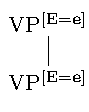
\includegraphics[scale=1]{VPcoerce.pdf}\hfill
\begin{forest}
[VP\textsuperscript{[E=\textbf{e}]}
  [VP\textsuperscript{[E=\textbf{e}]}]
]
\end{forest}\hfill
%  \end{minipage}
\caption{Frame and tree for coercion of an unbounded event into a bounded event \label{app:coerce}}
\end{figure}
